% assignment_5.text - Assignment 5 for Data Fusion class (Fall 2014)
% Chanmann Lim - October 2014

\documentclass[a4paper]{article}

\usepackage[margin=1 in]{geometry}
\usepackage{amsmath}
\usepackage{listings}
\usepackage{graphicx}

\everymath{\displaystyle}

\begin{document}
\title{CS 8790: Solution to assignment 5}
\author{Chanmann Lim}
\date{October 20, 2014}
\maketitle

\subsection*{Report:} ~\\
\indent The measurement state is a 3D estimate of the position of the target however the observations are obtained in lower dimensions (1D and 2D) with respective transformation matrix $H$. \\
\\
\indent The provided data come with a mixture of those 1D and 2D observations with the dimensionality value encoded at the beginning of each measurement. Thus, reading the dimension value(integer) is crucial to determine the numbers of subsequence data(floats) to be extracted to get a single observation. In the case that the observation is one dimensional the number of float values to read is $1+1+1\times3=5$, one value for mean $z$, one for covariance $R$ and $1\times3$ for the transformation matrix $H$. For 2 dimensional observation, the number of values to read from the data file is $2+3+2\times3=11$, two for the mean, three for the covariance and $2\times3$ for the transformation matrix.\\
\\
\indent After obtaining the observation, we can initialize the filter with the mean $x$ equals to zero and covariance $P$ to infinity(in Matlab code: use a very large number instead of INF) then combine them together using the fusion equation until all observations from the data file are fused.\\
\begin{align*}
x = \begin{bmatrix}
		0   \\  0   \\   0
	\end{bmatrix}, 
P = \begin{bmatrix}
		100000000   &  0   &   0 \\
		0   &  100000000   &   0 \\
		0   &  0   &   100000000
	\end{bmatrix}
\end{align*}
\begin{align*}
P_{new} &= P - WSW^{T}\\
x_{new} &= x + W(z - Hx)
\end{align*}
where
\begin{align*}
S &= HPH^{T} + R\\
W &= PH^{T}S^{-1}
\end{align*}
and the normalized innovation vector $v$ is
\begin{align*}
v = S^{-\frac{1}{2}}(z-Hx)
\end{align*}

\paragraph{1. } The plot of the normalized innovations (For the observation that provides 2 innovations, the first is being chosen for plotting):\\
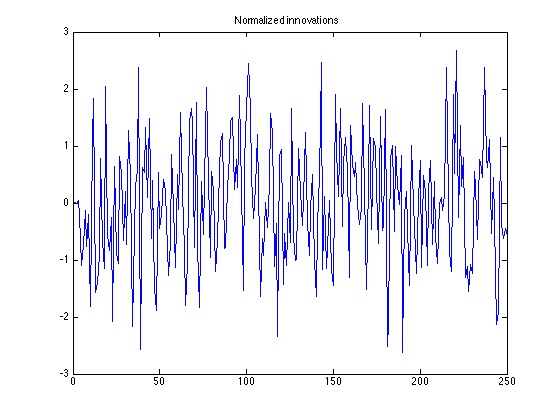
\includegraphics[scale=.75]{normalized_innovations.png}
\paragraph{2. } The plot of Randn with the same number of values as the above normalized innovations plot:\\
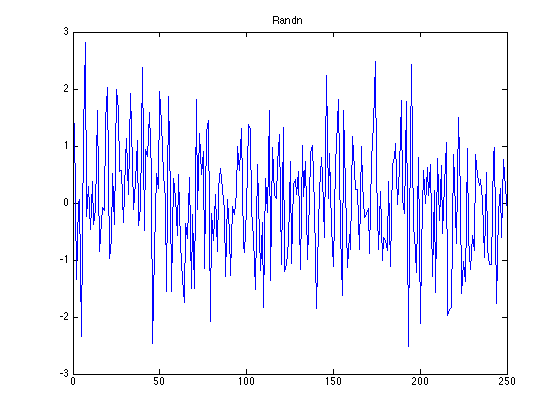
\includegraphics[scale=.75]{randn.png}\\

\paragraph{3. } The final mean $x$ and covariance $P$ are
\begin{align*}
x_{final} = 
	\begin{bmatrix}
		6.094090   \\   27.966840  \\   495.966545
	\end{bmatrix}
\end{align*}
\begin{align*}
P_{final} = 
	\begin{bmatrix}
        0.007794   &    0.000218   &    0.000258\\
        0.000218   &    0.007901   &    0.000107\\
        0.000258   &    0.000107   &    0.007835
	\end{bmatrix}
\end{align*}

\newpage
\subsection*{Appendix:}
\lstinputlisting[language=Matlab, title=\lstname, basicstyle=\footnotesize]{assignment_5.m}
\lstinputlisting[language=Matlab, title=\lstname, basicstyle=\footnotesize]{getObservation.m}
\lstinputlisting[language=Matlab, title=\lstname, basicstyle=\footnotesize]{update.m}

\end{document}